% !TeX spellcheck = cs_CZ
%{\tikzset{external/prefix={tikz/FYZI/}}
% \tikzset{external/figure name/.add={ch45_}{}}
%=========================== Kapitola: Ilustrace termodynamiky ====================================
\chapter{Ilustrace termodynamiky}\label{fyz:IchapXLV}
\minitoc
  \section{Vnitřní energie}\label{fyz:IchapXLVsecI}
  \section{Aplikace}\label{fyz:IchapXLVsecII}
  \section{Clasiova-Clapeyronova rovnice}\label{fyz:IchapXLVsecIII}
  \section{Příklady a cvičení}\label{fyz:IchapXLVsecIV}

    \begin{figure}[ht!] %\ref{fyz_fig463}
      \centering
      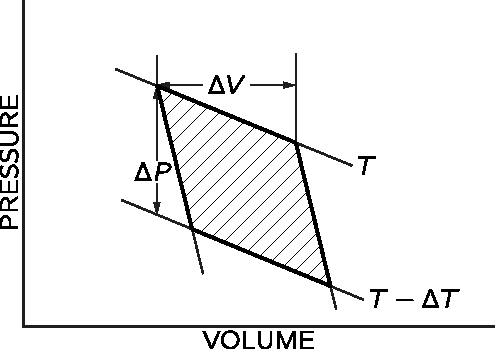
\includegraphics[width=0.7\linewidth]{fyz_fig463.pdf}
      \caption{ 
               (\cite[s.~707]{Feynman01})}
      \label{fyz_fig463}
    \end{figure}

    \begin{figure}[ht!] %\ref{fyz_fig464}
      \centering
      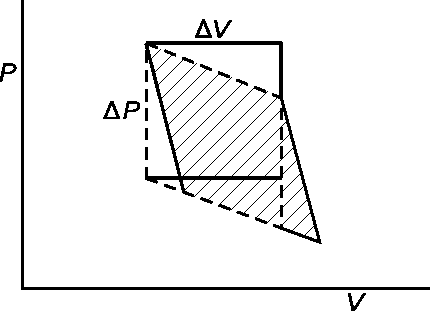
\includegraphics[width=0.7\linewidth]{fyz_fig464.pdf}
      \caption{ 
               (\cite[s.~707]{Feynman01})}
      \label{fyz_fig464}
    \end{figure}

    \begin{figure}[ht!] %\ref{fyz_fig465}
      \centering
      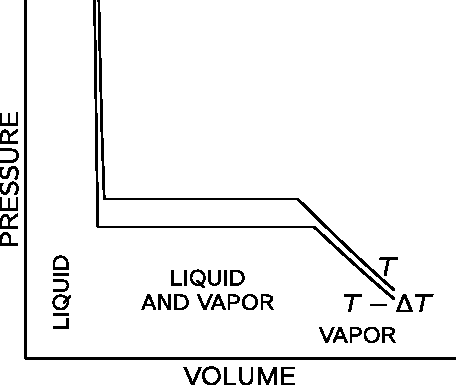
\includegraphics[width=0.7\linewidth]{fyz_fig465.pdf}
      \caption{ 
               (\cite[s.~707]{Feynman01})}
      \label{fyz_fig465}
    \end{figure}

    \begin{figure}[ht!] %\ref{fyz_fig466}
      \centering
      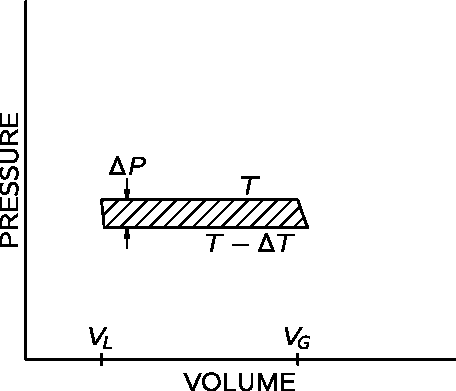
\includegraphics[width=0.7\linewidth]{fyz_fig466.pdf}
      \caption{ 
               (\cite[s.~707]{Feynman01})}
      \label{fyz_fig466}
    \end{figure}
    
%} %tikzset
%---------------------------------------------------------------------------------------------------
\printbibliography[title={Seznam literatury}, heading=subbibliography]
\addcontentsline{toc}{section}{Seznam literatury}